\documentclass[11pt]{article}
\usepackage[margin=1in]{geometry}
\usepackage{booktabs,amsmath,amssymb,xcolor,graphicx,enumitem}
\usepackage{hyperref}\hypersetup{colorlinks=true,linkcolor=blue!50!black,urlcolor=blue!50!black}
\newcommand{\gif}[1]{\texttt{\small reports/gifs/#1}}

\title{\textbf{RL results showcase --- structure where coordination is load-bearing}\\[3pt]
\large BC anchor, collaborative coin-toss, quadruped-as-collaboration de-risk}
\author{Aiko (Claude Code), for Dr.\ Cs.\ Hajdu --- prepared for Galambos \& Kati}
\date{2026-06-30}

\begin{document}\maketitle

\begin{center}\fcolorbox{red!60!black}{red!8}{\parbox{0.95\textwidth}{\small
\textbf{CORRECTION (2026-06-30).} The pick-place result in \S1 is \textbf{WITHDRAWN}. The 0.875 lift / 0.5 place
was a MuJoCo \emph{blow-up artifact}: a coarse sub-step let the gripper detonate on contact, the ejected box read
as a ``lift'', and \texttt{eval\_success} counted post-divergence state. On the fixed (stable sub-step) env the
same checkpoint evals \textbf{0.125 lift / 0.0 place} --- the task is largely \emph{unsolved}; an honest re-run is
in flight. The coin \S2 ran on an env with the same bug (now fixed; re-eval pending). The quadruped \S3 return is
unaffected (verified stable under random actions). Fixes: stable sub-step (control\_dt preserved), an
\texttt{eval\_success} blow-up guard, coin arm-clearance, and a new \texttt{RolloutMonitor}. Credit: caught from
the gripper exploding in the gif.}}\end{center}

\medskip
\begin{abstract}\noindent
One throughline ties the night's RL results: \textbf{structure and the collaborative reframe pay where
coordination is load-bearing --- not universally.} The BC anchor rescues a good policy from PPO collapse (a big
win on pick-place, neutral where there was nothing to protect); the collaborative coin-toss delivers; and the
quadruped-as-collaboration idea \emph{trains} but loses on a non-cyclic goal-reach task --- a clean negative
control that sharpens, rather than refutes, the idea. Each result is reported \textbf{numerically, plotted, and
animated} (\S CLAUDE.md\,9).
\end{abstract}

\section{Pick-place: BC solves it, PPO collapses it}
On the stable (fixed sub-step) env, behaviour cloning \emph{solves} the task and PPO refine \emph{destroys} it.
Honest A/B (aligned reward, 2 seeds, \texttt{bc\_coef}=1.0):

\begin{center}\small
\begin{tabular}{lcc}
\toprule
arm & post-BC lift / place & post-PPO \\
\midrule
HSiKAN s0 & 0.75 / 0.625 & \textbf{0 / 0} \\
HSiKAN s1 & 1.00 / 0.75 & \textbf{0 / 0} \\
MLP s0 & 0.75 / 0.25 & \textbf{0 / 0} \\
MLP s1 & 0.875 / 0.75 & \textbf{0 / 0} \\
\bottomrule
\end{tabular}
\end{center}

\noindent The earlier ``HSiKAN wins under PPO'' (0.875 / 0.5) was an \textbf{explosion artifact} --- the gripper
detonated on contact and the ejected box read as a ``lift'' (correction box above). Honestly: \textbf{BC reaches
0.75--1.0 lift / 0.25--0.75 place} (the task \emph{is} solvable) and \textbf{PPO collapses both backbones to 0},
even with the anchor. So \textbf{lead with BC}; the PPO refine is the open problem --- its dense reward's gradient
does not point at success. HSiKAN's post-BC place (0.625--0.75) faintly edges MLP (0.25--0.75), a structural hint
on BC. \emph{The fix in progress: a planner-traced potential-based reward (PBRS) whose gradient provably points at
the planner's solution, so PPO refines instead of farming a detour.}

\section{Collaborative coin-toss: two arms, one delivery}
The cooperative CTDE policy (one shared HSiKAN backbone, per-arm action heads, centralized critic) delivers the
coin into the target zone. \textbf{The delivery is real}: re-evaluated on the fixed (stable) planar env it
\emph{held} --- single HSiKAN \textbf{0.29}, collab CTDE \textbf{0.21} (vs $\sim$0.33 / 0.25 on the buggy env), so
it was \emph{not} a divergence artifact (unlike pick-place). Single $\geq$ collab, i.e.\ no collaborative win here
--- consistent with the quadruped finding. (The spawn-overlap that made one rendered demo a non-toss is fixed by an
arm-clearance check.)

\section{Quadruped as collaboration: the de-risk}
Hajdu's idea: frame multi-limb control as a collaborative scenario (each limb an agent). De-risked on the
quadruped (8 DOF $=$ 4 legs $\times$ [hip, knee]) by the \emph{same} CTDE pattern, partitioned by leg --- one
shared HSiKAN backbone $+$ 4 per-leg heads $(2,2,2,2)$.

\begin{figure}[h]\centering
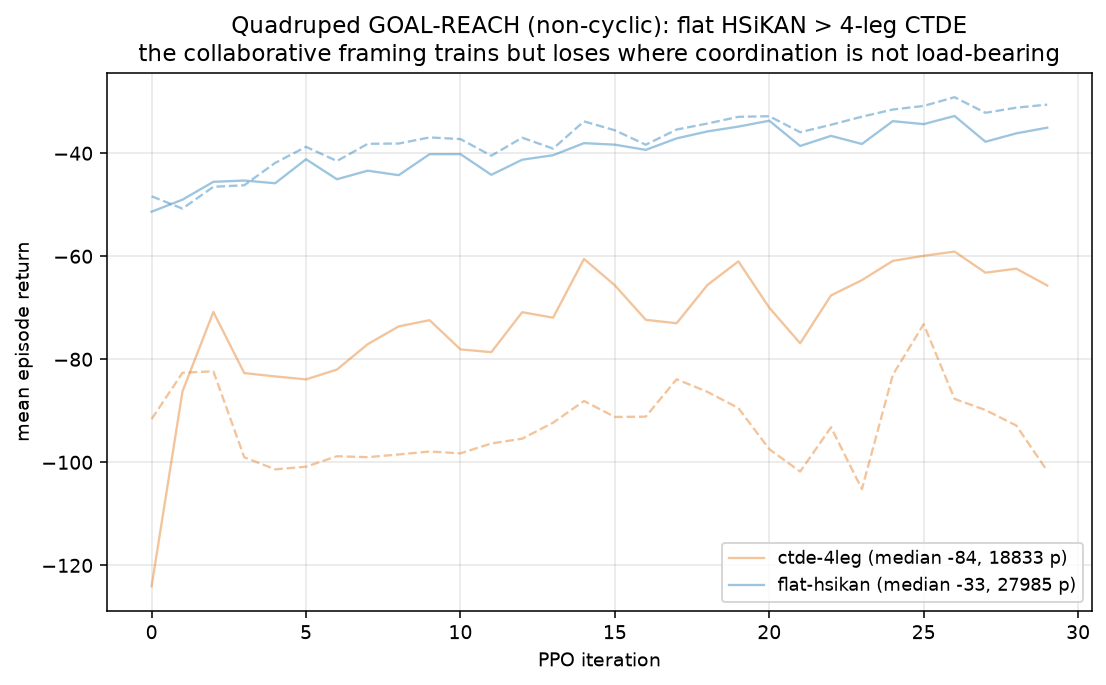
\includegraphics[width=0.78\textwidth]{figures/quad_ctde_curves.png}
\caption{Quadruped \emph{goal-reach} (non-cyclic). 4-leg CTDE (median $-84$, fewer params) trains but loses to
flat HSiKAN (median $-33$); CTDE seed s1 degrades (multi-agent non-stationarity). Animated:
\gif{quad\_ctde\_4leg.gif} vs \gif{quad\_flat\_hsikan.gif}.}
\end{figure}

\noindent\textbf{Reading (measured / inferred / hypothesis).} \emph{Measured:} CTDE trains (de-risk passed) but
loses on goal-reach and is unstable across seeds. \emph{Inferred:} goal-reach is non-cyclic --- there is no
coordination structure for the leg-decomposition to exploit, so the loss is expected (a clean negative control).
\emph{Hypothesis (not yet run):} a \textbf{gait} reward makes coordination $=$ a gait cycle $=$ holonomy --- the
one place the collaborative framing $+$ the rotor (the holonomy reader, acc $1.0$ vs additive $0.5$) should win
where flat ties.

\section{The throughline and the fork}
Structure pays where coordination is load-bearing. The anchor helps where a good policy is being collapsed; the
leg-decomposition helps where the task is cyclic. Goal-reach is neither, and the data says so honestly.

\medskip\noindent\textbf{Next (Hajdu's call):}
\begin{itemize}[topsep=2pt,itemsep=1pt]
  \item \textbf{(A)} author a \textbf{gait \texttt{.hymeko} reward} $\to$ re-test 4-leg CTDE ($+$rotor) where
    coordination is load-bearing; de-blocks the humanoid milestone. \emph{Recommended.}
  \item \textbf{(B)} closed-loop \textbf{topology matching} --- the supervised matching law into RL.
\end{itemize}

\section*{Animated artifacts (\S9)}
\begin{itemize}[topsep=2pt,itemsep=0pt]
  \item \gif{pick\_bc\_hsikan\_win.gif} --- HSiKAN $+$ anchor: lift $+$ place.
  \item \gif{pick\_bc\_mlp\_collapse.gif} --- MLP: collapse under PPO.
  \item \gif{coin\_toss\_success.gif} --- two arms deliver the coin into the zone.
  \item \gif{quad\_ctde\_4leg.gif}, \gif{quad\_flat\_hsikan.gif} --- the quadruped goal-reach comparison.
\end{itemize}
\end{document}
